\documentclass{sigchi}

% Use this command to override the default ACM copyright statement
% (e.g. for preprints).  Consult the conference website for the
% camera-ready copyright statement.


%% EXAMPLE BEGIN -- HOW TO OVERRIDE THE DEFAULT COPYRIGHT STRIP -- (July 22, 2013 - Paul Baumann)
% \toappear{Permission to make digital or hard copies of all or part of this work for personal or classroom use is      granted without fee provided that copies are not made or distributed for profit or commercial advantage and that copies bear this notice and the full citation on the first page. Copyrights for components of this work owned by others than ACM must be honored. Abstracting with credit is permitted. To copy otherwise, or republish, to post on servers or to redistribute to lists, requires prior specific permission and/or a fee. Request permissions from permissions@acm.org. \\
% {\emph{CHI'14}}, April 26--May 1, 2014, Toronto, Canada. \\
% Copyright \copyright~2014 ACM ISBN/14/04...\$15.00. \\
% DOI string from ACM form confirmation}
%% EXAMPLE END -- HOW TO OVERRIDE THE DEFAULT COPYRIGHT STRIP -- (July 22, 2013 - Paul Baumann)


% Arabic page numbers for submission.  Remove this line to eliminate
% page numbers for the camera ready copy 

%\pagenumbering{arabic}

% Load basic packages
\usepackage{balance}  % to better equalize the last page
\usepackage{graphics} % for EPS, load graphicx instead 
%\usepackage[T1]{fontenc}
\usepackage{txfonts}
\usepackage[natbib=true]{biblatex}
\addbibresource{Dissertation.bib}


\usepackage{times}    % comment if you want LaTeX's default font
\usepackage[pdftex]{hyperref}
% \usepackage{url}      % llt: nicely formatted URLs
\usepackage{color}
\usepackage{textcomp}
\usepackage{booktabs}
\usepackage{ccicons}
\usepackage{todonotes}
\usepackage{soul}

% llt: Define a global style for URLs, rather that the default one
\makeatletter
\def\url@leostyle{%
  \@ifundefined{selectfont}{\def\UrlFont{\sf}}{\def\UrlFont{\small\bf\ttfamily}}}
\makeatother
\urlstyle{leo}

% To make various LaTeX processors do the right thing with page size.
\def\pprw{8.5in}
\def\pprh{11in}
\special{papersize=\pprw,\pprh}
\setlength{\paperwidth}{\pprw}
\setlength{\paperheight}{\pprh}
\setlength{\pdfpagewidth}{\pprw}
\setlength{\pdfpageheight}{\pprh}

% Make sure hyperref comes last of your loaded packages, to give it a
% fighting chance of not being over-written, since its job is to
% redefine many LaTeX commands.
\definecolor{linkColor}{RGB}{6,125,233}
\hypersetup{%
  pdftitle={SIGCHI Conference Proceedings Format},
  pdfauthor={LaTeX},
  pdfkeywords={SIGCHI, proceedings, archival format},
  bookmarksnumbered,
  pdfstartview={FitH},
  colorlinks,
  citecolor=black,
  filecolor=black,
  linkcolor=black,
  urlcolor=linkColor,
  breaklinks=true,
}

% create a shortcut to typeset table headings
% \newcommand\tabhead[1]{\small\textbf{#1}}

% End of preamble. Here it comes the document.
\begin{document}

\title{Supporting Collaborative Information Analysis: A Classroom Study}

\numberofauthors{3}
\author{%
  \alignauthor{1st Author Name\\
    \affaddr{Affiliation}\\
    \affaddr{City, Country}\\
    \email{e-mail address}}\\
  \alignauthor{2nd Author Name\\
    \affaddr{Affiliation}\\
    \affaddr{City, Country}\\
    \email{e-mail address}}\\
  \alignauthor{3rd Author Name\\
    \affaddr{Affiliation}\\
    \affaddr{City, Country}\\
    \email{e-mail address}}\\
}

\maketitle

\begin{abstract}
% % abstract

Collaborative information analysis involves strategic analysis and representation of complex information space through synchronous and asynchronous team interactions over extended time periods. Chances are rare to observe how technology mediates team analysis over extended period of time because complex scenarios are difficult to model in lab studies, and professional analysts are limited to access in real world. Classroom study provides a testbed in which students are trained to become professional analysts and course projects are designed to simulate real world tasks. We developed a tool, CAnalytics, which aims to integrate data modeling and data analysis, and to support activity awareness amid demanding cognitive tasks. We deployed our tool in class and observed the usage of the tool by teams in their project. The paper reports the findings and discusses design implications.
%
%Collaborative information analysis typically involves representation and analysis of complex information space through synchronous and asynchronous team interactions over extended time periods. It is important to examine, understand, and provide effective tools and environments for these long-term, real world CSCW interactions. We have developed a tool, CAnalytics, to support collaborative information analysis through coordinated multiple views, to raise user awareness through real time sharing and other mechanisms, and to facilitate communication with an enhanced messaging tool. We deployed CAnalytics in an intelligence analysis course, in which 76 analysts-in-training used our tool for a one-week-long project. We report users' experience in this paper. Participants found the tool facilitated their teamwork and increased their engagement, but they also experienced breakdowns. The paper ended with discussion over design implications we derived from the field study.
\end{abstract}

\keywords{Collaborative information analysis; visualization; classroom study;}

\category{H.5.3.}{Information Interfaces and Presentation
  (e.g. HCI)}{Computer-supported cooperative work} 

\section{Introduction}\label{introduction}

Intelligence analysis is a form of sensemaking wherein a team of analysts
identify and evaluate causal relationships in a complex corpus of documents. A
common example of such an analysis is the investigation of a crime, where a variety of putative facts are assembled, e.g.
financial records, witness observations and interviews, and the social
connections between persons of interest. Armed with these different assembled facts
 investigators collaboratively: assess means, motives,
and opportunities; articulate and investigate further hypotheses and deductions;
and develop one or more theories of the crime.

%\bvh{Outline the critical challenge of modeling data and basing hypotheses on
% it. Current tooling forces you into waterfall.} \bvh{I would say the waterfall
% point first, and be more explicit about how it forces you into that model.}

According to Pirolli and Card's model \cite{Pirolli2005}, intelligence analysis
starts with modeling data from textual documents, followed by representing these
data models in various information artifacts, and developing them into
hypotheses.  Systems that currently support intelligence analysis are aimed at a
single phase and therefore only support part of the overall analysis workflow.
This imposes a clear boundary between each of these phases on the analysts. For
example, the Analysis of Competing Hypotheses (ACH) tool assumes that data has
been modeled, and that relevant evidence can be adduced appropriately to various
hypotheses, but provides no structured support for either. Other techniques,
such as Information Extraction and Weighting (IEW), help structure evidence
modeling, but do not extend utilization of evidence to hypothesis generation.
The unintended boundary between phases has the consequence that data modeled in
one software cannot be effectively utilized in hypothesis development in another
system. And analysts have to handoff, often via replicating the data in the new
system, information between software systems, making it difficult to revisit and
revise the data model. We therefore are motivated to develop an integrated
workspace in which analysts can model and analyze data in one place, and we
utilize the system as an experimental instrument to investigate analytic
behavior afforded by such integration.

% \bvh{Talk about how it is collaborative.} \bvh{Although I get lost in what you
% are trying to do in the end of this paragraph...I am not sure what point you are
% trying to make. This is the most confusing part of the intro so far}
Any intelligence analysis activity, at least at a non-trivial scale, is
fundamentally collaborative \cite{Convertino2011}. The intelligence community
puts great value on collaboration. A report from the Director of National
Intelligence, \emph{Vision 2015},  called for \emph{``a dramatic shift from
traditional emphasis on self-reliance toward more collaborative operations''}
\cite[p.13]{Vision2015}. However, most analytic tools that are widely used in
the intelligence community (e.g.~Analyst's Notebook \cite{IBM} and PARC ACH
\cite{PARC}) do not support collaboration. The community has to rely on separate
collaboration tools (e.g.~email, Intellipedia \cite{Intelink2017}), which lack
serious support for analytics, for team coordination \cite{Treverton2016}. Thus,
analysts must coordinate their work outside of their tool support, manually
sharing their analytic products.

Supporting collaboration in intelligence analysis is challenging, and perhaps
more than other situations (e.g.~collaborative writing, wiki) because the task
itself can be extremely complex. A team could be working with much more complex
data structure (e.g.~spatial data, temporal data, and relational data, as
opposed to text only), coordinating through multiple analytic artifacts
(e.g.~visualizations as opposed to document only), and making
sense of different levels of analysis, assumptions, and hypotheses, both
synchronously and asynchronously throughout a long-term course of collaborative
interaction. Thus teams must not only stay aware of what other members are doing, but \emph{why} they are doing that in a specific context of analysis. This study aims to investigate how technology can mediate team collaboration and to understand what awareness is needed beyond team actions.

%\bvh{Talk about what we did, this makes sense.}
We performed our study within the context of an intelligence analysis course.
This classroom study provides a natural environment in which participants engage
in multi-session, relatively complex class projects. Due to the difficulty in
accessing professional analysts due to security and confidentiality issues,
studying \emph{analysts-in-training} provides us a chance to include them in a
longitudinal design loop. These students already have knowledge and experience
with state-of-the-art analytic techniques and tools and are thus more likely to
provide insightful feedback. Besides, the students are young learners that are
willing to employ new work practices supported by features in tools. They are
important parts of the future intelligence community. In some sense, their
practice can be treated as a view into the future of practice of the community
\cite{Martin2014}.

We are thus motivated to investigate the feasibility, effectiveness and
consequence of supporting collaborative intelligence analysis in the context of
classroom study. We have developed a tool that includes annotation for data
modeling, interactive visualization for data analysis, and collaboration
features. While this paper reports a collaborative task in a specific domain,
findings regarding team process and breakdowns meet the interest of the broader
CSCW community. This study makes three contributions: 1) we observed a
spontaneously adopted interleaving workflow and quantitatively proved that an
earlier switch from modeling to analysis improved performance; 2) we
distinguished three collaboration strategies, five factors that impacted
performance, and issues that caused team breakdown; and 3) we explored further
the design of awareness support and proposed awareness surpasses simply teams
actions but includes contribution value, uncertainty, and context of insight.


\section{Related work}\label{related-work}

\subsection{Information analysis workflow}

Pirolli and Card's Think Loop Model \cite{Pirolli2005} is a widely used model of information analysis. The model describes the process of information foraging and sensemaking in which raw evidence is successively modeled, filtered, and synthesized into a best hypothesis. The model is a bottom-up process of structure building, but also includes a local feedback loop at each stage. Thus, analysts can reconsider propositions in the evidence file, asking how they are related, or a given hypothesis, asking what schemata it rests upon.

Empirical studies of information analysis suggest that the iterative looping can
have a wider scope than is obvious in the Pirolli and Card's model
\cite{Pirolli2005}. For example, Chin et al. \cite{Chin2009} observed five
professional intelligence analysts working both individually and as a team. They
found that analysts often need to review the original documents even at advanced
stages of analysis. The scope of these reconsiderations is not consistent with
the local feedback architecture of the Think Loop Model. It seems more
consistent with a parallel or multi-phased model \cite{Wheaton2011} in which
structure building occurs at a variety of levels in parallel. Similar findings
were reported by other empirical studies
\cite{Isenberg2008b,Kang2011,Herrmann2013a}. A report \cite{Badalamente2005}
from a workshop of professional intelligence analysts listed ``dynamic data
processing and visualization'' as one of top requirements in computational
support for intelligence analysis, emphasizing the need for an integrated
environment for data modeling and analysis.

However, tools supporting information analysis are often designed targeted at a single phase of activity, and thus not supporting the whole workflow. For example, research efforts have been made to understand information collection and modeling \cite{Shah2014i, Jansen2010c}, but little support is provided to extend these models to analysis. Techniques such as Information Extraction and Weight (IEW) helps structures data evidence but offers no structure to turn the evidence to hypothesis development. Similarly, tools supporting the activity of data analysis assume data has been modeled. Analytic tools such as interactive visualization emphasize present data in insightful means but provides no utility to data re-modeling \cite{Ware2012}.

Similar calls were made in other data intensive task domains as well. For
example, in interactive machine learning, researchers \cite{Chen2016,
Amershi2015} call for an all-in-one environment in which machine learning
practitioners can tune model parameters and evaluate model performance through
visualization in one place. In the area of visual analytics, Ware
\cite{Ware2012} warned of the \emph{``asymmetry in data rates''} [p.382],
pointing out that visual analytic tools emphasized data flowing from systems to
users far more than from users to systems. Functionalities are mostly designed
to adjust data representation rather than modeling, which are in fact equally
important. Our work aligns with these efforts, and contribute to the design and
evaluation of an integrated workspace in supporting information analysis tasks.

\subsection{Collaboration and awareness in information analysis}

Collaboration is critical in information analysis. The intelligence community has called for collaboration, and indeed closer collaboration, as opposed to merely coordinating draft products by the end \cite{Vision2015}. Empirical studies \cite{Chin2009,Kang2011} reported that analysts' practice was fundamentally collaborative. Effective collaboration helps analysts pool different knowledge and expertise and reduces the effect of confirmation bias \cite{Heuer1999}.

Significant efforts have been made to understand and support collaboration in the CSCW community, and many of them address, as it is in our study, tasks with large and complex data, such as collaborative modeling \cite{Kolfschoten2008, Prilla2013}, collaborative information seeking \cite{Golovchinsky2009a, Kelly2014a}, and collaborative visualization \cite{Isenberg2011,Heer2008e}. While these works provide insight in supporting teamwork with complex artifacts, less is known in terms of how technology-mediated collaboration occurs in a complete analytic process, and what awareness is needed for analytic specific purposes.

The state-of-the-art computational tools supporting intelligence analysis either
do not support collaboration, or they do not integrate serious analytic
support. On one hand, most analytic tools (e.g.~Analyst's Notebook and PARC ACH)
are designed for single user only, with only a few exceptions (e.g.~Te@mACH
\cite{Globalytica2017}). On the other hand, as Treverton \cite{Treverton2016}
reviewed state-of-the-art collaboration tools in the intelligence community, those
tools only support coordination for general situations, without specific analytic functionalities. For example, Intellipedia
\cite{Intelink2017} is a wiki platform for sharing of intelligence reports and
documents, yet it does not integrate functions for data modeling and analysis at all.

A key enabler for effective collaboration is \emph{activity awareness}, defined as
team's awareness of its own sustained collaborative activity
\cite{Carroll2003,Carroll2006}. Derived from Activity Theory \cite{Leontev1974},
activity awareness encompasses information covering all aspects of collaboration, such as partner presence, mediating artifacts, group actions, social interactions, shared information, and group values and norms. Activity awareness has been utilized as a design concept in guiding and evaluating collaboration features.

% place system figure here simply for paper layout
\begin{figure*}
\centering
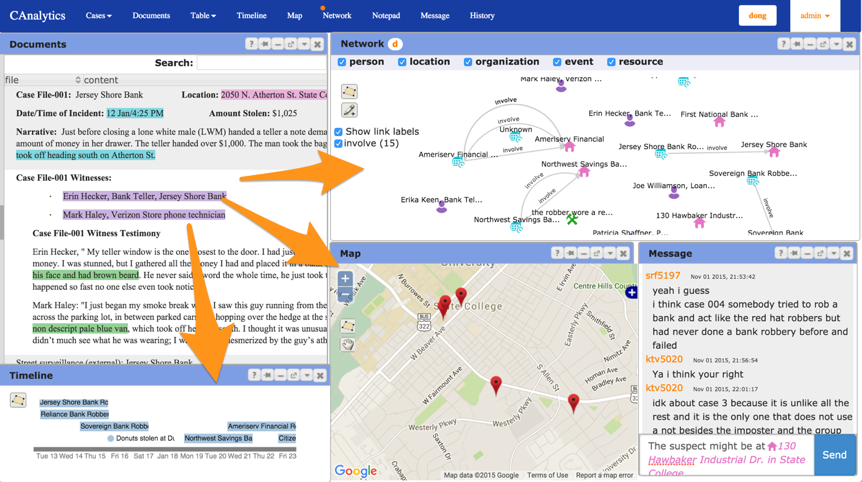
\includegraphics[width=2\columnwidth]{./img/interface.png}
\caption{CAnalytics user interface. Each window is closable, movable, and resizable. Shown here are \emph{document} view (top left), timeline (bottom left), network (top right), map (bottom middle), and message (bottom right). Other windows include table, notepad, and history view. }\label{fig:canalytics}
\end{figure*}

Many lab studies have been reported to investigate specific awareness features
to support collaboration in information analysis. For example, Convertino et al.
\cite{Convertino2011} examined the use of public and private views for role
based collaboration. Goyal and Fussell \cite{Goyal2016} studied the effect of
hypotheses sharing on sensemaking. Mahyar and Tory \cite{Mahyar2013b} designed a
visualization to connect collaborators' common findings and evaluated its
support for team performance. Hajizadeh et al. \cite{Hajizadeh2013} explored how
sharing teammate's interactions affects awareness. These studies provide
evidence to validate hypotheses of specific design features. However, due to
time constraint (mostly within one hour), these studies had to employ a
simplified task with reduced content and complexity. Artifacts created by
participants were thus relatively simple and superficial (e.g.~with a single
artifact or few items in an artifact). More complex task would have pushed
participants to create more sophisticated artifacts (e.g.~multiple views or
cluttered display that requires filtering) and to engage in a more dynamic and
complex workflow. Our study aims to examine team flow in a classroom context,
which allows for higher task complexity and longer teamwork time in a more
realistic environment, and thus provides opportunities to gain more insights
into team-based analytic process. .


\section{CAnalytics Features}\label{canalytics-features}


%\bvh{I think that the biggest thing missing from here is an argument about *why* they tool has been built the way it is. This should really link up to the arguments that you made in the abstract/intro about dynamism and collaboration more explicitly.}

As shown in Figure~\ref{fig:canalytics}, we developed a web application tool, \emph{CAnalytics} (standing for ``C-ollaborative Analytics''), to
support teams of analysts in identifying, visualizing, integrating and
assessing facts from multiple sources. Two particular design objectives are 1) to build an integrated environment for intelligence analysis, and 2) to support collaboration with shared data and awareness functions. The design is informed by earlier
paper prototype studies \cite{Borge2012, Carroll2013}, in which the researchers examined team's communication patterns and
spontaneously created artifacts in a crime scenario. We also take into account findings from
empirical studies conducted by Chin et al. \cite{Chin2009} and Kang
and Stasko \cite{Kang2011} when making design decisions.
%\bvh{I would mention the reasons why we built it again here as an organizing structure for introducing the features and how they relate to those two overriding goals of dynamism and collaboration - modified}

\paragraph{Coordinated multiple views for data modeling and analysis}

To enable an integrated environment for different functionalities of analysis, CAnalytics employs a multiple-view interface, with each view in a floating, closable window. Views are coordinated and share the underlying data pool so that products of different activities are not fragmented. The following paragraphs describe features of each view.

The \emph{document} view supports evidence modeling through annotation. Annotation provides a basic structure to assist analysts in containing and framing new data. In the
document view users can select and highlight a snippet of text and
annotate it as a type of entity such as a person, location, event, etc.,
or as a relationship between entities. Unlike other entity-based
systems such as \cite{Bier2010,Stasko2008}, we use annotations to
allow analysts to manually create evidence objects of interest. Manual
annotation allows for greater user control in terms of
information of interest and granularity that best suits their ad-hoc
analytic needs.
%\bvh{I wouldn't make too big of a point out of not supporting automated analysis, I would instead put it as something to look at in future work. You are sort of calling out a whole couple of fields in this set of statements. - modified}
Users can add attributes to the annotated object, e.g.~time in an event, and coordinate in a location. Users can
also make reference to other objects in the attribute; for example,
users can add people objects to an event indicating that these people
were involved in the event.
%\bvh{I almost think this is too fine grained of a description...you could just take the first sentence or two of this and add it to the previous paragraph. -deleted some}

These annotations turn text into structured data objects, which are then displayed in visualizations in the same workspace, including \emph{table}, \emph{timeline}, \emph{map},
and \emph{network} view---artifacts that are frequently constructed to hold attribute
data, temporal data, spatial data and relational data respectively
%\bvh{not sure what point you are trying to make here}
\cite{Carroll2013}. Figure~\ref{fig:canalytics} shows an example:
when an annotation is created in the document view with information
about time, location, participants, and their relationships, a new event
is created in the timeline view, a new location is created in the map
view, and new people are added to the network graph with a labeled edge
representing the relationship (or new edges are added to existing
nodes). Hovering the mouse over an entity will activate an entity detail
window that displays attributes in detail, and analysts can modify, or
re-model the entity in situ.

The views afford brushing and linking interactions;
that is, when users brush entities in one view, related
entities are displayed in other views. Thus the analyst can narrow down
entities to their interest by: specifying a time range using the functionality provided on the timeline; making a spatial query
with map filter; or selecting a cluster of entities by drawing a bounding
area in the network view.

\paragraph{Collaboration and awareness features}

To support collaboration, CAnalytics affords real-time collaborative editing, similar to the
Google Tools. Users can open several concurrent editors to
collaboratively edit multiple entity objects. Entities and annotations are immediately
shared within a team and rendered in teammates' corresponding views.

In addition to real-time data sharing, CAnalytics supports other awareness features. A \emph{notification system} sends
individual's actions to the team in the form of a text box located in the top
right corner of the workspace. An iconic
indicator on top of a view window, which we call \emph{tool coordinator}, shows who else is also working on this view. A \emph{message} tool is a real time chat window that enables team
communication with persistent message history. The system also maintains
a traceable log of time-stamped individual activities in the \emph{history} tool.
Users can learn team activities about who did what to which object at
what time. Entities mentioned in the message tool and
history tool are hyperlinked and will trigger pop-up detail window when
the user moves the mouse over them. With these awareness features, users who work
synchronously can be informed of others' activity continuously; users
who work asynchronously will be able to use the history to reconstruct
their work status and become aware of changes beyond the point of their
last interaction.



\section{Classroom Study Settings}\label{classroom-study-settings}

The context for this study was an undergraduate course in an
intelligence training program in a US university. The program was
designed to train students to become professional intelligence analysts.
A key requirement of the course is to emphasize hands-on practice on
team-based intelligence analysis. During the first nine weeks, students
learned strategic knowledge (e.g.~bottom-up analysis and top-down
analysis) and structured analytic techniques, such as IEW, ACH and
network analysis, and practiced to apply these techniques to solving two
small projects with state-of-the-art tools including PARC ACH and IBM
Analyst's Notebook.

Our study began from the 10th week of the course and lasted for one
week. The task was to investigate a series of bank robberies fabricated
by the course instructor. Teams were provided with a set of documents
pertaining to seven robberies, including police reports, witnesses
reports, video records, and news media. The task was designed
open-ended, which meant that there was no single answer to the task. The
instructor explained that the task was to simulate real world scenarios,
in which analysts always reasoned in the circumstances of uncertainty,
ambiguity, and complexity. The instructor told the students that 6 hours
was expected to complete the project, including in-class and
outside-class work. In the end of the project students were required to
submit a team report, describing their hypotheses, assumptions,
conclusions and supporting evidence.

Students were given a tutorial on CAnalytics a week before the project
began. One of the authors walked through features of CAnalytics and then
let students accomplish a small case analysis on their own pace. During
the study week, one author was always available to help with any
technical issues. Although students were encouraged to make full use of
CAnalytics, to ensure a naturalist environment students were always free
to employ any other tools that they believed useful.

Of the 98 students enrolled in the course (from two sections), 73
consented to participate in the study. Students were randomly assigned
into 25 teams (23 three-person teams and 2 two-person teams). Research
suggested that group size be an important factor in group collaboration,
thus two-person teams might behave differently from three-person teams.
We thus excluded data from the two-person teams in our analysis in this
paper. Also, from the log (and confirmed by their questionnaire), we
found that one team made little use of CAnalytics and opted for other
tools (Google Doc). Hence their data was also excluded. Thus in this
paper we reported the result from 22 teams.

All the students held major in the program of Security and Risk
Analysis. Most (75\%) of them were in the third academic year (3.05
years in average), indicating that participants in our study had
relatively advanced experience and knowledge in intelligence analysis.
Participants' age ranged from 19 to 28 (20.3 in average). 77\% of the
participants were male.

We employed several data collection approaches. We administrated a
post-study questionnaire, which included several 7-index questions
measuring individual's self-reported awareness (adapted from
\autocite{Convertino2011}), team communication (adapted from
\autocite{Convertino2011}), collective efficacy (adapted from
\autocite{Convertino2011}), perceived performance (adapted from
\autocite{Goyal2014}), and cognitive load \autocite{Hart1988}. The
questionnaire also included open-ended questions asking how the tool
helped or impeded their work. We captured user interactions with system
logs. Instead of simply logging low-level events like mouse click and
keyboard strokes, we recorded actions such as making an annotation and
deleting an entity. Finally, we reviewed team reports and graded them as
an indicator of team performance. We designed an assessment rubric
together with the course instructor.




\section{Results}\label{results}

While participants could access the tool any time, teams had three most
intensive usage sessions over the week: two were in class and one was outside
class before the team report deadline. 22 teams self disclosed that they used
CAnalytics as the principle analytic tool throughout the project although they
were free to use others; one team reported that they mostly used Google Doc
because they \emph{``felt more used to''}. Nine other teams reported having used
Google Doc, but only for composing the final team report. Seven teams reported
using GroupMe and other instant message outside class. They used these tools for
instant communication and coordination of meeting. Thus the CAnalytics system logs captured
most of team's analytic sessions, although their communication data could be
partially missing.

Over the week, teams created 1805 entities and 1529 relationships in
total. The number of entities teams created ranged from 24 to 223 ($M=82,
SD=39.9$), and the number of relationships ranged from 7 to 237 ($M=69.5,
SD=51.0$), showing a large variety. The big range was related to different team data modeling strategy,
which will be discussed in detail later.

CAnalytics was generally well received by the students. An overview of
the related survey items (shown in Figure~\ref{fig:survey}) shows that students positively rated all aspects
of the tool except cognitive load, towards which they had a close to neutral feeling. % \bvh{provide more detail here, don't just rely on the figure}

\begin{figure}
\centering
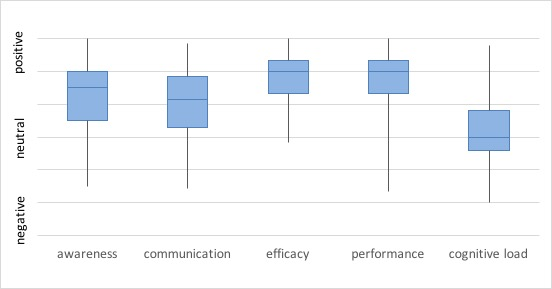
\includegraphics[width=3.00000in]{./img/survey_boxchart.jpg}
\caption{Survey responses (box shows Q1-Q3 and median; ends of whiskers show
maximum and minimum)\label{fig:survey}}
\end{figure}

\subsection{Interleaving data modeling and analysis}\label{interleaving-data-modeling-and-data-analysis}

%\bvh{you need the reason why this is interesting...i.e. evidence of these behaviors shows that the tool was used collaboratively}

%\bvh{also what exactly do you mean by interleaving ... you should probably give an example or something??? maybe not, up to you}

We examined the pattern of data modeling and analysis first by
qualitatively looking at a visualization of the entire interaction log
(e.g.~Figure~\ref{fig:interleaving}a shows one team's interaction). All teams
worked intensively on data modeling as they started off the project.
This was the phase when teams were getting themselves familiar with the
documents and made initial annotation input into CAnalytics. Starting from certain
time point, all teams started analysis on visualizations,
followed by frequent transitions between data modeling and analysis. 11
teams started data analysis in the first usage session, while the other
11 teams had this transition in the second usage session. In average,
the transitions occurred in 47.6 minutes after the project began. The earliest transition occurred in 14 minutes after the team started the project, and the last team
had the transition around 104 minutes, later in the second session. We
also found performance difference among teams that started analysis
early and those late. Teams that started analysis in session one had
higher performance ($M=8.6$) than teams that started from session two
($M=6.7$), although the difference was not statistically significant.

The fact that participants returned to making annotations after analysis
indicated that they did not wait to start analysis till they had
finished modeling. Indeed, the activity of data modeling and data
analysis were highly interleaved throughout the project (as shown by the interleaving color bar in Figure~\ref{fig:interleaving}a). Participants switched from
one activity to the other activity frequently. The state transition
diagram (Figure~\ref{fig:interleaving}b) demonstrates the interleaving in an aggregated way, in which we
encode the number of transitions as width of the link. This result
confirms our design expectation that data modeling and analysis should
not be supported as separate staged activities, and that an integrated
environment should streamline the workflow.

After confirming the existence of interleaving workflow, we explored further what drives the switching between data modeling and analysis. We looked into team behavior in modeling and analysis respectively through log analysis and artifact analysis, and describe the results below.

\begin{figure*}
\centering
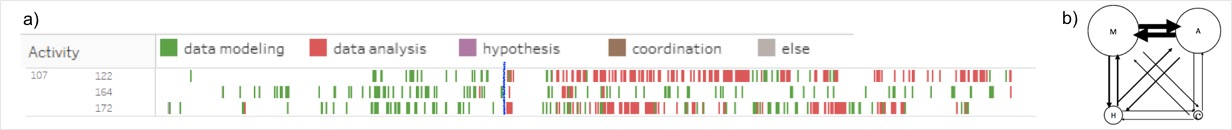
\includegraphics[width=6.5in]{./img/intertwined.jpg}
\caption{(a) Visualization of interaction logs of Team 107. Each row of
colored marks indicates the sequence of top level activities a
participant performed. (b) State transition diagram of interaction logs of Team 107. Each node is an activity, whose size represents the time spent on the it (M: data modeling; A: data analysis; H: hypothesis development; C: coordination); a
link represents a switch from one activity to another, whose width
encodes the number of switches. We see highly frequent transitions between data modeling and data analysis \label{fig:interleaving}}
\end{figure*}


\subsection{Data modeling: filtering vs.~accretion}\label{data-modeling-accretion-vs.filtering}

\begin{figure}
\centering
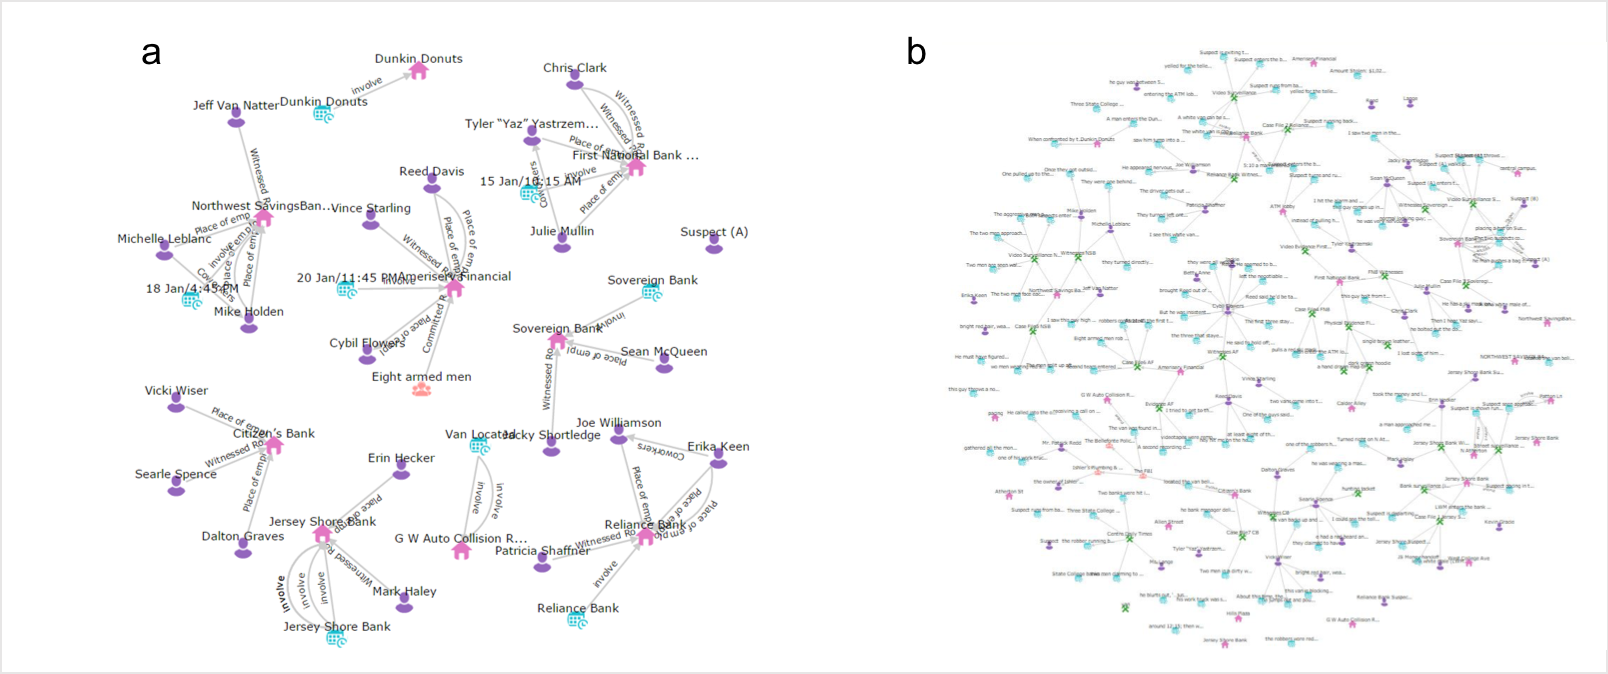
\includegraphics[width=\columnwidth]{./img/network_accretion_filter.png}
\caption{Network artifact comparison: filtering (a)
vs.~accretion (b) \label{fig:network_accretion}}
\end{figure}

We noted a distinction between filtering and accretion
strategies in data modeling, similar to what was reported in a paper prototype study \cite{Carroll2013}. Filtering is selectively modeling of data
and adding to an artifact. Users must decide what information is
relevant, and thus what is to be excluded, as well as what granularity
of information is to model. Filtering requires more team coordination,
because teammates must reach a common ground of the current problem as
well as information needed to answer the problem. Figure~\ref{fig:network_accretion}a is an example of network built with filtering strategy. It only represented key information of robberies and thus provides a good overview of the whole story.

Accretion is an attempt to comprehensively represent the problem by adding
information of all levels of details to an artifact. Users extract every fact
from the document, regardless of its immediate relevance to the problem.
Accretion requires less coordination as it is relatively mechanical note taking.
A disadvantage of accretion is that the produced artifact could be fairly
complex. An example is Team 108, who modeled every step the suspects took in a
robbery. Such artifact provides a detailed view of the data, and can be useful
when a step-by-step comparison is needed to identify robbery patterns. Yet it
also resulted in far more entities (223) than the average (82) and more
cluttered network view (Figure~\ref{fig:network_accretion}b). This accounted for
the large range of entities created across teams mentioned beforehand.
Participants also realized the problem. They reflected that they spent too much
time in detail events, and many did not help their analysis at all:

\begin{quote}
\emph{I felt that after we were done annotating, we hadn't really accomplished
anything and that we were no closer to solving the case than when we had
started. In the end it didn't really help that we had annotated the
data. (P86)}
\end{quote}

Filtering and accretion strategies are not exclusive; in fact many teams applied a mix of two strategies. Depending on the need of analysis, filtering provides an overview of the whole story, and accretion helps investigate a specific robbery in detail. Modeling data at different levels opens different analytic threads, which accommodates multilevel analysis, including examining attributes of an individual entity, comparing two related events, and developing a hypothesized story on the whole dataset.

\subsection{Artifact analysis: fact
vs.~inference}\label{artifact-construction-fact-vs.inference}

\begin{figure}
\centering
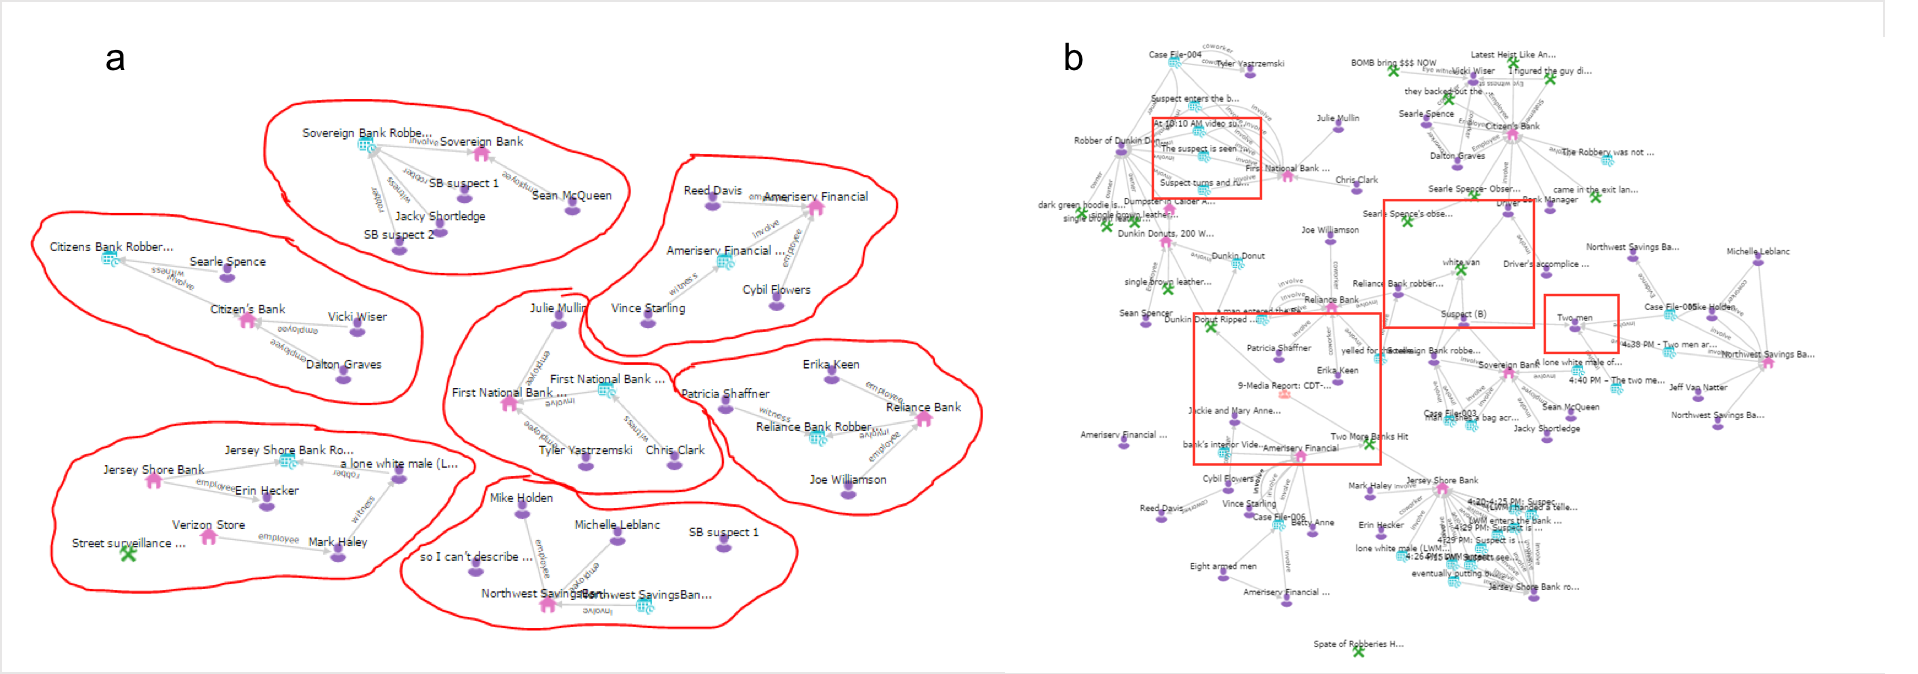
\includegraphics[width=\columnwidth]{img/network_cluster.png}
\caption{Network artifact comparison: separate clusters (a)
vs.~connected clusters (b). The parts highlighted in red squares in (b) are key
evidence that connects clusters\label{fig:network_cluster}}
\end{figure}

We examined the analytic artifacts teams created, the network
graph in particular because social relationships played the most
critical role in this specific scenario and teams spent most time on
network analysis (as reflected from the log). We found a clear distinction among the network artifacts. For example, networks from
8 teams ($\text{mean performance score}=7.8$) consist of separate clusters
%\bvh{-I don't think you say what is good and what is bad though??-yes, in the end of settings section -do you ever describe what the performance means?}
(Figure~\ref{fig:network_cluster}a). Nodes within a cluster are
connected, representing information space of a robbery case; Nodes
between clusters are nonetheless not connected, indicating each robbery
is a self-contained case. However, these these teams did not miss the connections between robberies, as these teams still discussed these robbery connections in their report.
It turned out that these teams documented any possible relationships between
robberies in the notepad tool as a list, separate from the network graph; that is, these teams distinguished information content and synthesized them in different artifacts.
%\bvh{add something, but still not powerful enough yet -what does this have to do with anything? I think you need a sentence here saying what this means, you don't explain this until 2 paragraphs later}

In contrast, 6 other teams ($\text{mean performance score}=8.3$) created networks
composed of connected clusters. While a cluster is still a
representation of a robbery, some of them are connected through an
evidence node. An example is Figure~\ref{fig:network_cluster}b, in
which we mark in red four \emph{connectors} that link the clusters. These
connectors were key evidence that led the teams to hypothesize that
those robberies were related and might be committed by the same criminal
group (e.g. the white van shown up in two robberies). These teams represented all information in one artifact.
%\bvh{how about this - same comment, outline what it means in a sentence and then tie them together like you do in the next sentence.}

By comparing these two types of networks, we found that links within a cluster were typically
\emph{factual} relationships modeled from raw documents (e.g.~a white van was
witnessed at a location), and links between clusters were often
\emph{inferences} beyond literally documented (e.g.~a white van at location A
is the same van witnessed at location B). Teams creating separate
clusters represented only facts in the network and held evidence with
uncertainty in a separate artifact. One advantage of distinguishing
facts and inferences is that teams can always be aware of assumptions made when
making a conclusion. And since all inferences are held in one place,
teams are forced to confront them and review their uncertainty
iteratively in the process. However, the strategy also adds difficulty
to analysis as analysts may overlook or fail to combine evidence
scattered in different artifacts.

% place table simply for paper layout
% Please add the following required packages to your document preamble:
% \usepackage[table,xcdraw]{xcolor}
% If you use beamer only pass "xcolor=table" option, i.e. \documentclass[xcolor=table]{beamer}
% \usepackage[normalem]{ulem}
% \useunder{\uline}{\ul}{}
\begin{table*}[]
\centering
\small
\label{tab:awareness}
\begin{tabular}{p{3cm}p{10cm}}
\rowcolor[HTML]{9B9B9B}
\multicolumn{1}{c}{\cellcolor[HTML]{9B9B9B}\textbf{Element}}                           & \multicolumn{1}{c}{\cellcolor[HTML]{9B9B9B}\textbf{Example}}                                                                                                                                                                                                                                                                                                                                 \\
\rowcolor[HTML]{C0C0C0}
\begin{tabular}[c]{@{}l@{}} Social awareness\\ \emph{who is present?}\end{tabular}             & CAnalytics helped me stay aware,of my teammates activities because I could see who was logged on in the top,right corner (P123)                                                                                                                                                                                                                                                              \\
\rowcolor[HTML]{EFEFEF}
\begin{tabular}[c]{@{}l@{}}History awareness\\ \emph{Who has done what?}\end{tabular}         & The way you are able to view when and where your teammate made or updated annotations/information was the key to staying aware of what your team has done. It is a great tool in respects to that. For example, I was able to view the changes my team made while I was not using the CAnalytics tool at the same time they were using the history tab. (P171)                               \\
\rowcolor[HTML]{9B9B9B}
\begin{tabular}[c]{@{}l@{}}Information awareness\\ \emph{What is being changed?}\end{tabular} & CAnalyitics was very helpful in keeping us updated on what was being changed/noted/amended by whom and when. This was very beneficial for staying on the same page and knowing what changes were being made so no one individual was out of the loop. (P157)                                                                                                                                 \\
\rowcolor[HTML]{EFEFEF}
\begin{tabular}[c]{@{}l@{}}Action awareness\\ \emph{Who is doing what?}\end{tabular}          & I liked how you could always see what your teammate were viewing on the website. For example I was working on the bluf when my teammates were working on the network part of the program. If I were to come across a piece of information that I thought might be helpful to them I would just tell them. My teammates did the same thing in return. (P51)                                   \\
\rowcolor[HTML]{C0C0C0}
\begin{tabular}[c]{@{}l@{}}Intention awareness\\ \emph{Who is going to do what?}\end{tabular} & CAnalytics showed what tab {[}tool{]} my teammates were working on which helped me be aware of what they were working on. For example, if I saw that one of my teammates was on the network tab, I knew that they were attempting to connect the information that was relevant to one another.,I would then be able to mention any new findings I had that could influence their work (P160)
\end{tabular}
\caption{Subject feedback of awareness instances}
\end{table*}


On the contrary, in connected-cluster networks, facts and inferences overlaid in one artifact together drive the layout of the
network, are better synthesized, and give analysts a clearer picture in one place. Teams may discuss and evaluate the level of uncertainty of inferences to decide whether to add them to the
network. This strategy makes analysis more interactive among teammates:
they need to negotiate, evaluate, and reach consensus on the value and
validity of inferences. However, a problem with mixing facts and inferences is, to some extent teams might forget whether a
link is factual or inferred, and ask whether conclusion derived
from the visualization can be trusted under uncertainty.

Uncertainty in analysis represents a gap between analyst's knowledge and data needed to address the problem. The existence of uncertainty drives analysts to switch to data modeling and to collect more data or remodel existing evidence in order to resolve the uncertainty.

\subsection{Collaboration and
awareness}\label{collaboration-and-awareness}

One recurring theme in the subject feedback we collected was that the
collaboration features were helpful for solving the problem. In the survey
88\% of the students positively rated their
group awareness. Participants appreciated that the tool complemented
traditional analytic tools, describing CAnalytics as Analyst's Notebook with real time
synchronization features similarly to Google Docs, or described it as Google Doc with added visual analytics. To quote one participant,
\emph{``CAnalytics is like an analysts notebook that multiple people
could work on at once {[}\ldots{}and{]} an analysts version of a Google
Doc'' (P65)}.

Participants reflected that they could now contribute simultaneously
without concerns of interference and could
have everything in one place instead of manually sharing documents via a
cloud service.

\begin{quote}
\emph{It was much easier to coordinate as a team with CAnalytics because we
could all work on the same system at the same time. Without CAnalytics,
we were forced to do the work separately and compile all the work onto
one system after we had finished. (P156)}
\end{quote}

Students also reported that being able to see teammate's status made the
task more motivating and engaging:

\begin{quote}
\emph{During class I wasn't sure if my teammates were doing work for that
class or another thing but then seeing their dot {[}tool indicator{]}
switch between applications on the software and updates pop up on my
screen I knew they were doing work for 231. (P141)}
\end{quote}

\begin{quote}
\emph{The fact that you can see what other teammates are doing and they can
see what you are doing creates a sense of accountability in terms of
separating the work load. (P51)}
\end{quote}

The motivating effect of awareness might account for, at least partially,
the fact that teams were participating equally. We measured the equality of
participation in terms of number of created entities and time spent on
CAnalytics. We refer to Olson \cite{Olson2017} in calculating equality: one
minus the variance of proportions times 100 (for better readability). Thus
the score ranges from .67 (when only one person contributes in a three-member
team) to 1.00 (when everyone participated exactly equally), and higher
score indicates higher balanced participation. The resulted equality of
created entities and time was .96 and .99 in average respectively. This
indicates participants contributed fairly evenly.

Another repeated theme was the awareness features helped assure all teammates were executing
the team plan. Participants reflected on their experience that a common
team breakdown was misunderstanding of the team plan, and that they did
not realize the misunderstanding until everyone had spent significant efforts
finishing their ``perceived'' job. CAnalytics made plan execution assured
because they could always see where teammates were working and what they
were generating; and if anything unexpected happened, they could communicate
immediately rather than in the end of the project.

Participants reported many other instances of awareness they realized
using CAnalytics. We categorized them based on the element of awareness,
or the essential problem of awareness of \emph{what}
\cite{Schmidt2002}, into social awareness, information awareness,
action awareness, history awareness, and intention awareness, as shown
%in Table~\ref{tab:awareness}. somehow shown in Table 5.4
in Table 1.

When asked what features helped them stay aware of team activities, 28
participants mentioned the tool coordinator, 24 mentioned the
notification system, 19 mentioned the history tool, 14 mentioned the
real-time update of user-generated data, 12 mentioned the collaborative
editor, and 7 mentioned the message tool. Although the number of mentions
does not simply indicate tool usefulness, it suggests users were explicitly aware of these awareness features and appreciated their support.


Students' positive feedback on awareness was further corroborated by
interaction logs. For example, we measured the number of entities
accessed by other collaborators. While data
generated by users is automatically shared, it is up to collaborators
whether to read/edit the shared information or ignore information altogether.
The log showed that on average, 77.6\% of the created entities
were \emph{read} by at least one other teammate. Further, We measured how
many entities were \emph{edited} by collaborators, a phenomenon we argue
requires higher awareness, because the collaborator must not only realize
the creation of the entity, but also understand its content. We
defined \emph{peer editing}, manipulated as the ratio of editing other's
entities over editing those created by oneself. We found that all teams
edited collaborator's entity objects, with a peer editing value equal
to .83 ($SD=.45$). The result suggests that teams had little difficulty
accessing and modifying partner's created data objects.

%/bvh{I don't understand this paragraph...what are you trying to say...that they would like to have a shared space?}
One major critique is the lack of support for sharing intermediate analytic
insights. An insight is revealed and contextualized by a specific arrangement of views, e.g.~a reduced data view of interest through filter, a highlighted entity representing the analytic focus, and a clustering layout of network to demonstrate a specific relationship. While teammates share the same data pool, they are likely to have different views of data, and thus different \emph{interpretations}
toward the data. A dynamic view together with its interpretation represents
user's intermediate analytic status. Sharing these insights could inspire team analysis \cite{Gotz2009d}. With CAnalytics
participants complaint that they could not easily make such communications. The team could \emph{``be
looking at the same information but arranged in completely different
ways'' (P131)}.

\subsection{Labor division strategies}\label{labor-division-strategies}

We noted different labor division strategies from interaction logs. Seven
teams followed \emph{document-based collaboration} (DBC): they divided their
work by evenly distributing the different documents among team members
(as shown in Figure~\ref{fig:labor_division}a). Each member read
through and made annotations on their own set of documents. An advantage
of this strategy is that individuals get less workload and thus have
more time to think deeply about their own documents. Individuals also
implicitly take over the responsibility of their assigned documents to
gain insights and share them when the team synthesize findings in later
analysis. When the team needs information from one document, they rely
on the ``document owner'' to share his/her finding. The failing of this
strategy is thus in case an individual fails to identify or convey
evidence in the document, the team may overlook the information
altogether \cite{Borge2012}.

Four teams followed an \emph{entity-based collaboration} (EBC)
strategy. Instead of dividing by documents, they divided work by entity
types: each individual went through all documents but only annotated
entities of certain types, e.g.~teammate A only annotated persons and
teammate B annotated locations (as shown in
Figure~\ref{fig:labor_division}b). This strategy seems to save teammate's time in the
data modeling phase. And since each person focuses only on certain entities,
they are more likely to identify recurring patterns, for example, the
white van used in multiple robberies. However, focusing on certain
entities could lead individuals to superficial syntactic scanning of
documents instead of deep reading. This could further lead to extremes
of annotating all entities of the type, whether they are related to the
problem at hand or not, similar issues with accretion strategy discussed
beforehand. Indeed we found from the interaction log that EBC teams
created more entities ($M=101$) in average than DBC teams ($M=94.5$).
Moreover, with emphasis on certain entities,
individuals are likely to know only partial aspects of a robbery and
hence have difficulty connecting and synthesizing facts to deduce any
conclusion. As one participant reflected, \emph{``we broke up by entity
type, which reduced our individual involvement in each other's entity
types'' (P99).} The result indicated that the average performance of EBC teams ($M=7.63$) was lower
than that of DBC teams ($M=9.25$), although the difference was not statistically significant.

The rest (eleven) of the teams did not show specific labor division
patterns. Indeed, teams did not necessarily have to divide their work in
order to collaborate, especially when the collaborative tool provides
possibility to work closely together. Teammates could read and annotate
the same document because they could see new annotations by others in
real time and build on other's annotation. Figure~\ref{fig:close_collaboration}
shows an example where one team worked on the same document simultaneously.
The three team members exhibited high synchronicity in which document to
analyze, which we believe was not by accident. This has the advantage that
teammates are always on the same page and can discuss hypotheses
throughout the analysis process. Participants did have concern for
possible duplication. As one participant complaint, \emph{``we could not
actively see the changes our teammates were making until well after they
had made them'' (P46)}. This was because an annotation was shared only
\emph{after} it was created, yet another teammate might already be drafting an
annotation on the same text snippet in the meantime.

\begin{figure}
\centering
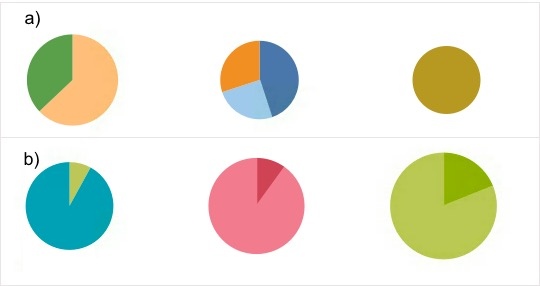
\includegraphics[width=3.20000in]{img/labor_division.jpg}
\caption{Pie charts showing different labor division strategies. Each
pie chart corresponds to one team member. (a) Document-based
collaboration. The pie chart shows the documents one team member
annotated, color coded by document ID. (b) Entity-based collaboration.
The pie chart shows the entity types one team member created, color
coded by entity types.\label{fig:labor_division}}
\end{figure}

\begin{figure}
\centering
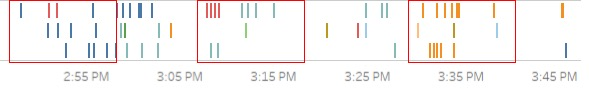
\includegraphics[width=3.20000in]{img/close_collaboration.jpg}
\caption{Graph showing the timeline of one team creating annotations.
Each row corresponds to one team member. Each bar represents an
annotation, color coded by document ID. The red blocks highlights the
periods when all teammates worked on the same documents
simultaneously.\label{fig:close_collaboration}}
\end{figure}

\subsection{Interaction with team performance}

To systematically evaluate factors that influenced team performance,
we conducted a multiple linear regression between team performance
as the dependent variable and team collaboration characteristics
(i.e.~equality of entities and time respectively, peer editing, number of entities created, shared
entities, switch time from data modeling to analysis) as independent
variables. We treated a team as a system \cite{Henman2003b} and modeled team-level
relationships.
The relationship of individual level variables (e.g.
survey items) could not be simulated with regression directly because data within a team was interdependent. The analysis was performed using \emph{R} \cite{R2016}.

The result is shown in Figure~\ref{fig:regression}. The regression model was found to be statistically significant ($F(5,16)=4.58; p<.01$), with an R squared equal to .59, meaning 59\% of the variability in team performance was explained by the model. Five team-level variables contributed significantly to prediction of team performance. The model suggested that balanced contribution of entities predicted higher team performance scores ($\beta=45.79, p<.05$), but balanced participation time did not show such effect. More peer editing led to better performance ($\beta=3.89, p<.01$), implying that analysts should be encouraged to model data as a team, and to remodel other's entity objects as needed. Longer elapsed time before a team started analysis (\emph{switch time} in the figure) predicted lower performance ($\beta=-.05, p<.05$), which suggested that teams should shorten the time of pure data modeling and start analysis earlier. Larger number of entities teams created also predicted higher performance ($\beta=.03, p<.05$). This can be interpreted that teams providing sufficient model input did benefit from system support. However, we are not ready to claim more entities are always better  because we should also be cautious that entities irrelevant to the team problem bear no value to team analysis, as discussed beforehand. Somewhat surprisingly, the number of shared entities negatively predicted performance ($\beta=-8.99, p<.05$).
%\bvh{hard to understand this sentence...not sure how to rewrite it.}
We considered this might also relate to the issue of entity value: sharing entities without relevance to the team problem leads to reduced team efficiency and creates distraction, which in turn would lead to worse team performance. Another possibility is that teammates may not necessarily access all entities partners created. The theory of Transactive Memory \cite{Wegner1987} suggests that teammates do not have to know everything in the team but should know ``who knows what''. Individuals specialize in their own field (e.g. one specializes in event analysis while another in social relationship examination) and reach for collaborators when other knowledge is needed. In such case, common knowledge in shared entities would actually be redundant. Individuals do not need to access content of entities created by others, but only keep aware of the creator.

\begin{figure}
\centering
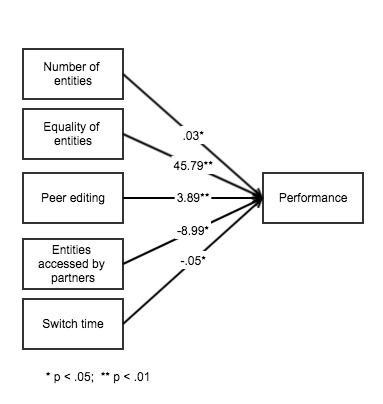
\includegraphics[width=3.0000in]{img/team_analysis.jpg}
\caption{The relationship between collaboration characteristics and team performance.\label{fig:regression}}
\end{figure}


\section{Discussion}\label{discussion}

The goal of the study is to understand and support an interleaved workflow in
collaborative information analysis by evaluating tool usage in a natural
environment over multiple usage sessions. Our work responds to calls for an
integrated environment made in the intelligence community as well as other data
intensive domains \cite{Shah2014i, Chen2016, Vision2015, Amershi2015, Ware2012}.
The system builds upon prior empirical studies (e.g. \cite{Carroll2013,
Borge2012,Kang2011,Chin2009}) and embodies their design implications in our
tool. The study also complements research that only tests tools in short term
lab studies (e.g. \cite{Convertino2011,Goyal2016,Hajizadeh2013}) by
investigating tool usage over multiple usage sessions.

This study adopts an \emph{analyst-centered design} approach. A critical
requirement of developing tools that meet user needs is to understand their
needs and practices. When these needs and practices are specialized (as is the
case in intelligence analysis), it is particularly important to include the
target user population in the design process \cite{Scholtz2014}. Our classroom
study provided an opportunity with deep access to analysts in training. These
analysts have been trained with knowledge and skills of intelligence analysis,
and have experience with state-of-the-art analytic tools such as Analyst's
Notebook and PARC ACH. In their reflections, participants often compared
CAnalytics to those tools. Their multi-session usage of CAnalytics also allows
them to adapt to the tool and learn to appropriate it to the best of their team
purpose \cite{Stahl2006}. Therefore, while their feedback is admittedly not the
same as an experienced professional, their feedback does provide a deeper
insight into strengths and weaknesses of CAnalytics.

The study provides encouraging results. Participants appreciated an all-in-one
environment where they could share raw documents, evidence snippets, views of
evidence and hypotheses in one place. They liked the fact that they could
contribute simultaneously without blocking or interfering each other. Another
benefit of the collaborative tool is to keep teammates aware of each other's
activities. Staying aware of teammates not only helps establish a common ground
for planning team strategy, but also ensure everyone is following the plan as
expected. Moreover, results suggest the awareness features provide positive
\emph{social facilitation} \cite{Zajonc1965}: individuals found the task
motivating and engaging with awareness of each other's activity. We also
measured collaboration characteristics that impacted team performance, and found
that balanced contribution, peer editing, and earlier switching from modeling to
analysis predicted higher team performance. Most importantly, we documented the
interleaved workflow enabled by the integrated environment, and explored
momentum in modeling and analysis behaviors that drove the activity switching.
Below we discuss design implications that could potentially enable a better
collaborative experience in information analysis tasks.

\subsection{Scaffold a structured interleaved workflow}

A misconception about information analysis is that data modeling and
data analysis are two staged activities. This is akin to the \emph{waterfall}
software development model, which features a sequential process that
flows downwards through the phases of requirement conception, software
design and implementation, and testing and maintenance. Critics have
argued against this approach and instead called for an iterative design
process that leads to reframe user requirements,
redesign, redevelopment, and retesting.

Our result demonstrates a similar iterative and dynamic process in information
analysis. The result is striking especially because our participants have been
trained with tools that impose a waterfall model. They could have followed their
old waterfall practice with our tool, yet instead all teams spontaneously
switched to an iterative manner. We projected that modeling on multiple granularities drives analysis on different levels, and uncertainty in analysis pushes analysts back to collecting additional data.

Realizing that, we probably could shape analysts into a more interleaved
workflow with a more structured approach. Structured techniques such as IEW and ACH  help users
perform analysis in a systematic and transparent manner in each well defined activity, yet fall short in guiding analysts in switching between the two activities
\cite{Kang2011}. Our system implies a structured modeling through annotation and
a structured analysis by visualizing data in multiple views. By sharing the same
data structure and consistent user interface, we enable a smooth switching
between the two stages. Our result implies the role of multilevel modeling and
analysis uncertainty in driving the switch. Based on that, there exist design
opportunities to enable a more interleaved flow. For example, we can build a more structured scaffolding process to bridge modeling and analysis. When user adds a
new data object, the system could suggest possible connections to existing
evidence in the context of an appropriate level of views, which is likely to
help analysts discover new patterns. When a user creates a new hypothesis with
uncertainty, the system could highlight associated evidence, which would prompt
the analyst to re-examine the data and look for more data. Such scaffolding
provides a basic structure to link stages of analytic activities that analysts
can take on without imposing a specific fixed workflow.

A smoothier interleaved workflow could also be made by increasing team
awareness of partner's modeling and analysis. That is, uncertainty in one's
analysis not only motivates oneself to data modeling, but also drives partners
(who is aware of the what and why of the uncertainty) to collect more data.
Similarly, one's modeling could influence and drive partner's analysis, given
the partner is fully aware of what is modeled and how the new data connects to
the level of existing data. Such ``team-level'' interleaving could make teamwork
more interactive and close coupling, but also requires support of higher
awareness, especially of hypothesis uncertainty and data model context. Improved
design for multi-granularity modeling, uncertainty representation, as well as
team awareness of these features opens up possibilities for coordinating
interleaving at the team level. We discuss these design implications in further
detail in the following paragraphs.

\subsection{Build collapsible views for multi-level modeling}

We observed that analysts built data models in multiple granularities and engaged and coordinated among different levels of details. For example, analysts jumped
quickly from digging into details of a single event, to comparing between two
events, and to overviewing all robberies as a complete story. When sharing these data, a critical requirement is to represent them in an appropriate context in order to ensure teammates understand them correctly. A collapsible data view could be a solution to accommodate such
multi-level modeling. This can help draw teammate's attention to a specific item
while keeping the global context available. Analysts can focus on a certain
level of detail at a time while conveniently switching between levels. A
collapsible view also reduces the problem of cluttered view when data volume
increases.  and when analysts dig into greater
details (e.g.~representing suspect's all actions to identify patterns of common
actions in two robberies). An analyst can overview all robberies and only unfold
detailed actions when investigating into a specific robbery.

\subsection{Design a richer graphic language for uncertainty}

Uncertainty is prevalent in analysis and more prevalent in collaborative
analysis because each teammate becomes a source of uncertainty when they
contribute a piece of information \cite{Chin2009}. Teams in our study
spontaneously employed two different approaches to deal with uncertainty: either
to mix them for better synthesis or to separate them for better clarification.
Representing uncertainty appropriately assures teammates when they build
analysis upon other's insight. This helps reduce the problem emphasized in Chin
et al.'s work \cite{Chin2009} that analysts do not trust partner's conclusion.
It also helps teammates stay aware of issues that need to be addressed, thus
decide what extra data is needed. We propose that a richer graphic language and
interaction be designed so that analysts can encode uncertainty into the views.
For example, links and entities with different uncertainty can be visualized in
different transparency. Users can \emph{filter} by uncertainty so that users can
choose to consider evidence only with high credibility, or to review all
inferences and decide what extra data is needed to consolidate them.

\subsection{Share views as team resource}

View sharing is important for sharing and understanding analytic result
\cite{Morton2014a}. A common solution is to enable a public view which always
keeps synchronized for all teammates \cite{Convertino2011,Greenberg1990}.
However, a single public view does not meet the need in intelligence analysis
because analysts may want to share multiple views in an iterative analysis
process. We propose that views should be treated as a \emph{team resource}, just
like data, which is sharable, extensible, and reusable. For example, an analyst
can save their current view as a shared resource when they feel it useful to
collaborators. Other people can reuse the view to their need. Shared views
should be interactive rather than static images, so that analysts can perform
all interactions including filtering and highlighting, and are able to evolve
the view with collective team efforts, a critical requirement emphasized in
\cite{Carroll2013}.

\subsection{Distinguish visible vs. valuable contributions}

Finally, we noted cases where teams created far more entities than needed with an
accretion strategy. Strikingly, while similar data modeling strategy was
reported in the paper prototype study \cite{Carroll2013}, users with CAnalytics
seemed far more tempted to accretively add information, with far more entities
and cluttered views. For example, the extreme team created as many as three
times entities than the rest teams in our study, much more than the difference
in the paper prototype study. Why did this happen? We guess both the context of
classroom study and the system design contributed. Unlike in the lab study where
teams are temporarily assembled, teams in a class evaluate peers either
consciously or unconsciously and value how themselves are being evaluated. Such
social pressure motivate individuals to make contributions, and indeed to make
\emph{visible} contributions, more than \emph{valuable} contributions. That is,
participants noticed that their work activity was visible to their partners, and
accordingly prioritized doing more visible work over doing less visible work. In
some cases, this led to a new problem of easy and less valuable contributions
that were highly visible - such as creating and therefore sharing data entities
that were not particularly important, and subsequently made data models seem
cluttered. For example, creating and therefore sharing an entity gets
immediately notified to the team whereas weighing the importance and relevance
of an entity goes silent in the system. We need to investigate approaches to
making significant contributions more visible, or perhaps making it more
immediately visible that less important contributions are indeed less important.



% \section{Conclusion}
\hl{not modified yet}

% Limitation
In this paper, we present findings from a classroom study in which teams of information analysts in training collaboratively completed a complex intelligence project mediated by our tool. As collaborative information analysis is increasingly a typical and chronic task, it is important for research to examine, understand, and provide effective tools and environments for these long-term, real-world CSCW interactions. This requires situating research in more complex work activity contexts, and directly investigating interactions, experiences, and outcomes in those contexts. Our classroom study provides initial results on team interactions mediated by advanced technology over extended time periods. The encouraging results motivate us to continue refining and re-evaluating the tool.

Meanwhile, due to the nature of classroom study, a lot of variables that cannot be factored could influence the result. For example, students coordinated teamwork not only through CAnalytics but also through face-to-face meeting. What the teams did outside CAnalytics is not collected, which obviously influenced team performance. But our work provides a realistic picture of usage of a collaborative tool in real world, and poses several design questions and hypotheses, which could be investigated in future controlled lab studies. 

%Since the study was conducted in a naturalist environment, participants were not observed in a controlled lab, and they were free to choose either face-to-face collaboration settings or remote work settings, and they could also use any other tools they preferred. Thus their high rating of awareness in the survey is not a sufficient proof of the success of the tool. Still, their answer in the open-ended questionnaire explained to some extent how the tool helped achieve the function.  
%
%
%establish the dots and connect the dots
%
%
%
%This paper talks about strength and weakness of lab and field study, and suggests combining the two methods. 
%A laboratory method for studying activity awareness. Convertino. 2004

\section{Acknowledgments}

To be added

% Balancing columns in a ref list is a bit of a pain because you
% either use a hack like flushend or balance, or manually insert
% a column break.  http://www.tex.ac.uk/cgi-bin/texfaq2html?label=balance
% multicols doesn't work because we're already in two-column mode,
% and flushend isn't awesome, so I choose balance.  See this
% for more info: http://cs.brown.edu/system/software/latex/doc/balance.pdf
%
% Note that in a perfect world balance wants to be in the first
% column of the last page.
%
% If balance doesn't work for you, you can remove that and
% hard-code a column break into the bbl file right before you
% submit:
%
% http://stackoverflow.com/questions/2149854/how-to-manually-equalize-columns-
% in-an-ieee-paper-if-using-bibtex
%
% Or, just remove \balance and give up on balancing the last page.
%
\balance{}


% REFERENCES FORMAT
% References must be the same font size as other body text.

\printbibliography

\end{document}

%%% Local Variables:
%%% mode: latex
%%% TeX-master: t
%%% End:
